\documentclass[12pt]{report}
\usepackage{thesis}
\usepackage[dvipdfmx]{graphicx}
\usepackage{url}
\usepackage{amsmath}
\usepackage{tabularx}
    \newcolumntype{C}{>{\centering\arraybackslash}X}
    \newcolumntype{L}{>{\raggedright\arraybackslash}X}
    \newcolumntype{R}{>{\raggedleft\arraybackslash}X}
\usepackage{subfigure}
\renewcommand{\bibname}{Reference}
\title{Watercolor Image Generation Based on Diffusion Model}
\author{Banglin Zhang}{M225163  }
\eauthor{Banglin Zhang}
\school{Graduate School of Advanced Science and Engineering, }
\major{Hiroshima University}
\adviser{Prof. Koji Nakano}
\date{ September 2024}{August 2024}
\begin{document}
\maketitle



\begin{abstract}
With the development of deep learning, the application of deep learning in image generation is becoming more and more widespread. Especially the generation of images in various special styles, such as oil painting style, sketch style and watercolor style. However, existing research on watercolor style image generation is often achieved by style conversion, which limits the creative ability of the model. At the same time, the models do not simulate the watercolor effect well.

In this study, in order to solve the above problems. Firstly, a high-quality watercolor image dataset is produced and used for model training. In order to achieve the purpose of generating high quality watercolor images. Starting from Vision Transformer and diffusion model, this study abandons the U-Net structure commonly used in diffusion model and redesigns the network structure of diffusion model based on Vision Transformer. Compared with the existing model, the quality of watercolor image generation is improved.
\end{abstract}
\newpage

%%%%%%%%%%%%%%%%%%%%%%%%
%%%%  諸設定  %%%%%%
%%%%%%%%%%%%%%%%%%%%%%%%
\pagenumbering{roman}
\tableofcontents
\listoffigures
\newpage
\pagenumbering{arabic}

%%%%%%%%%%%%%%%%%%%%%%%%%%
%%%%  ↓ここから本文  %%%%
%%%%%%%%%%%%%%%%%%%%%%%%%%



\chapter{Introduction}
\section{Research Background}
The rapid development of deep learning techniques has not only led to remarkable achievements in the traditional fields of computer vision and natural language processing, but has also demonstrated its potential in the creation of art. One notable application is the use of deep learning to generate watercolor images, which provides a whole new dimension to digital art. Watercolors are known for their distinctive brushstrokes, soft color transitions, and unique style of the artist, and deep learning techniques are able to simulate and reproduce this traditional art form in an unprecedented way. However, due to the characteristics of watercolor images, popular deep learning generation models often fail to achieve satisfactory results. This has driven the development of specialized generative network architectures for watercolor image generation. To meet the needs of artistic creation, film and animation production, or custom product design, this study aims to achieve the generation of high-quality watercolor images. We created a high-quality watercolor image dataset and designed a new network specifically for the task of watercolor image generation.

With the rapid development of deep learning techniques, image generation tasks are gradually categorized into two main research areas. As shown in Figure \ref{fig:intro} , label-based image generation and image generation based on input images \cite{isola2017image}. Most of the deep learning generation models on watercolor images before this are graph-generated tasks, and very few of them are based on label generation \cite{wang2023stroke}. This does not allow the model to be innovative and stochastic, whereas models for artistic creation like watercolor images. It is in line with the demand to make the model appear artistic and abstract generation appropriately. Therefore, this study revolves around label based generation of watercolor images.

\begin{figure}[h]
    \centering
    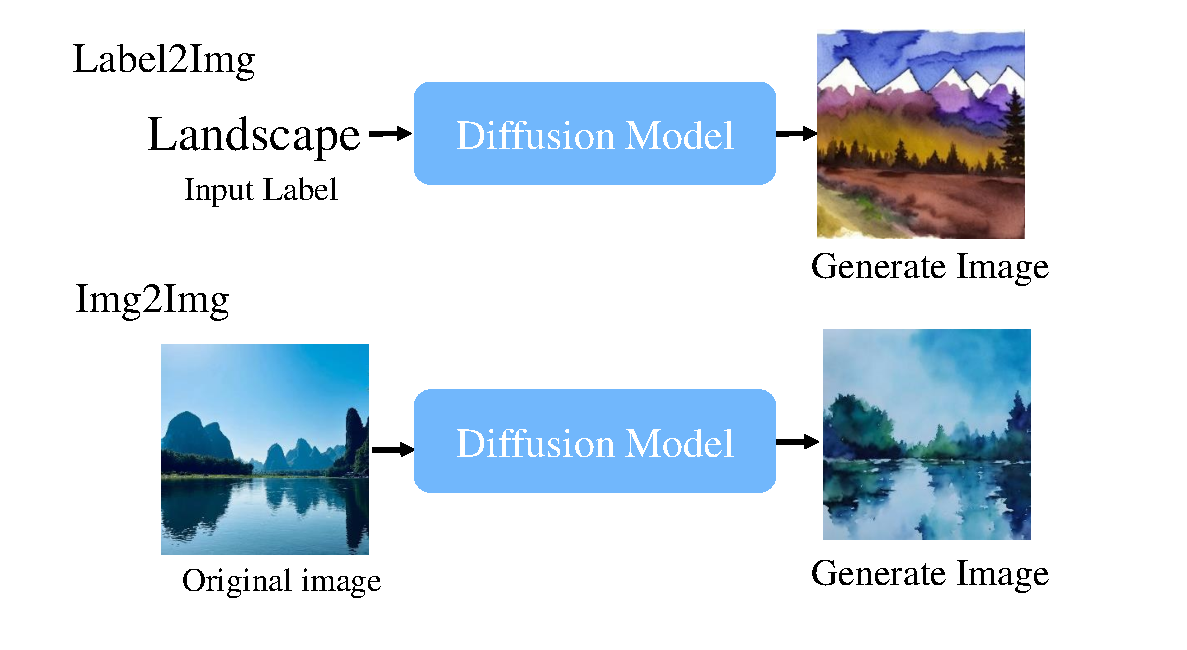
\includegraphics[width=14cm]{image/intro.pdf}
    \caption{Different image generation methods}
    \label{fig:intro}
\end{figure}

Additionally, the network structures used in this study are categorized based on their characteristics. The current mainstream generative models include Generative Adversarial Networks (GAN) \cite{goodfellow2020generative} and diffusion models. Among these, GAN have gained attention due to their widespread application but face several issues such as mode collapse, making it challenging to generate high-quality images. Given these challenges, this study decided to abandon the use of GAN in favor of the more stable diffusion models. Diffusion models generate high-quality and diverse images by progressively adding noise to the images and learning the denoising process. Compared to GAN, diffusion models perform better in terms of stability and generative effects, and they are better at reconstructing and simulating the characteristics of images.

Diffusion models can maintain high levels of detail and structure when generating images, preserving the original image's texture and color transitions. Through this method, we aim to simulate the characteristics of watercolor paintings, including color blending, edge blurring, and texture effects, to ensure that the generated watercolor images exhibit excellent visual and artistic qualities.

In the diffusion model U-Net is widely used, U-Net is a network structure proposed in 2015, which was first used for image segmentation tasks \cite{ho2020denoising}\cite{ronneberger2015u}\cite{rombach2022high}. Due to its excellent performance it was soon ported to other domains. However, when the diffusion model with U-Net structure is used to generate watercolor images, problems such as unclear targets occur. Therefore in this study, in order to improve the generation of watercolor images, we give up the use of U-Net structure, and design the diffusion model backbone network structure from scratch based on the inspiration of Vision Transformer and other models \cite{dosovitskiy2020image}, in order to achieve the purpose of generating high-quality watercolor images.

\section{Research Purpose}
We aim to develop a model that generates watercolor images based on given labels. Figure \ref{fig:proposedModel} shows our proposed method for generating watercolor images. In this example, the model generates a watercolor image of a dog from random noise based on the input label (dog). To achieve the research objectives, we first plan to collect a dedicated watercolor dataset, which will include various categories of watercolor paintings. Specifically for watercolor image generation, we will design a deep learning model architecture aimed at developing a model capable of generating high-quality watercolor images that comprehensively simulate the characteristics of watercolor paintings.

\begin{figure}[h]
    \centering
    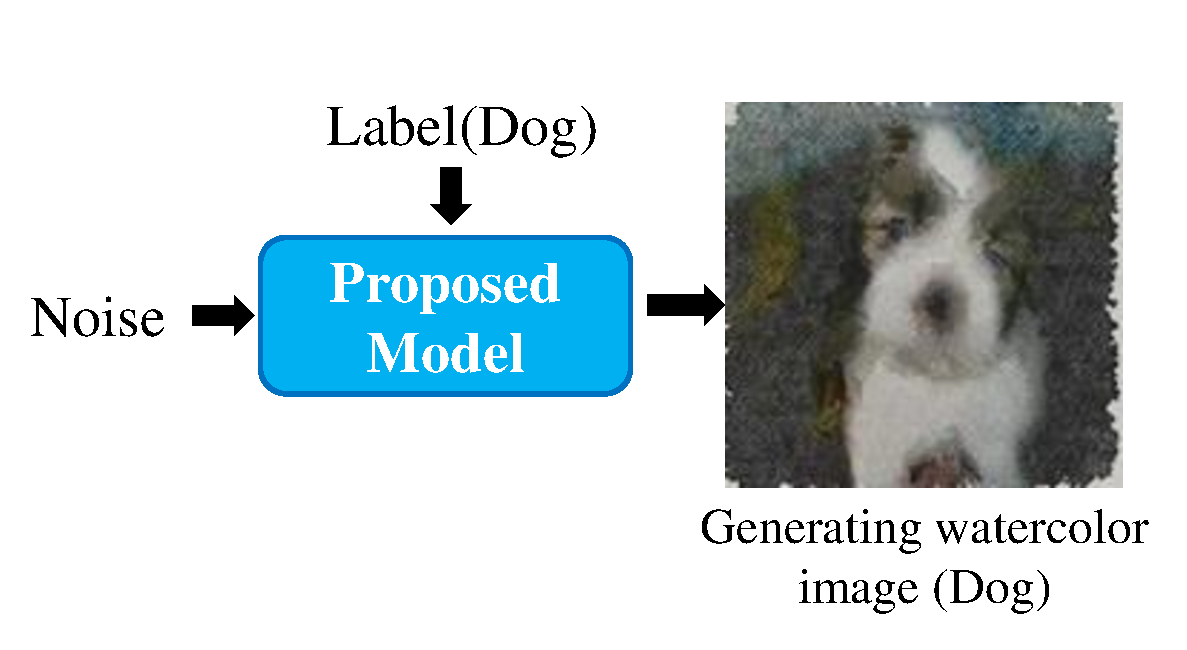
\includegraphics[width=12cm]{image/proposedModel.pdf}
    \caption{Proposed method for generating watercolor images}
    \label{fig:proposedModel}
\end{figure}

\section{Chapter Structure}
The other chapters are presented below. Chapter 2 begins with a description of the related work. Chapter 3 describes the dataset used and the methodology used for its collection. Then, Chapter 4 describes the methodology proposed in this study. Finally,  experiments and conclusions.


\chapter{RelatedWork}
\section{Diffusion Model}
The key idea of Diffusion Probabilistic Models \cite{ho2020denoising} is to gradually evolve a simple noise distribution into a target data distribution through a diffusion process. Specifically, the basic assumption of Diffusion Probabilistic Models is that an initial simple probability distribution, usually Gaussian (Gaussian noise image). It gradually evolves into a target data distribution (Generated image) through a series of probabilistic diffusion steps. This process can be accomplished by iteratively applying the diffusion operation. 
\begin{figure}[h]
    \centering
    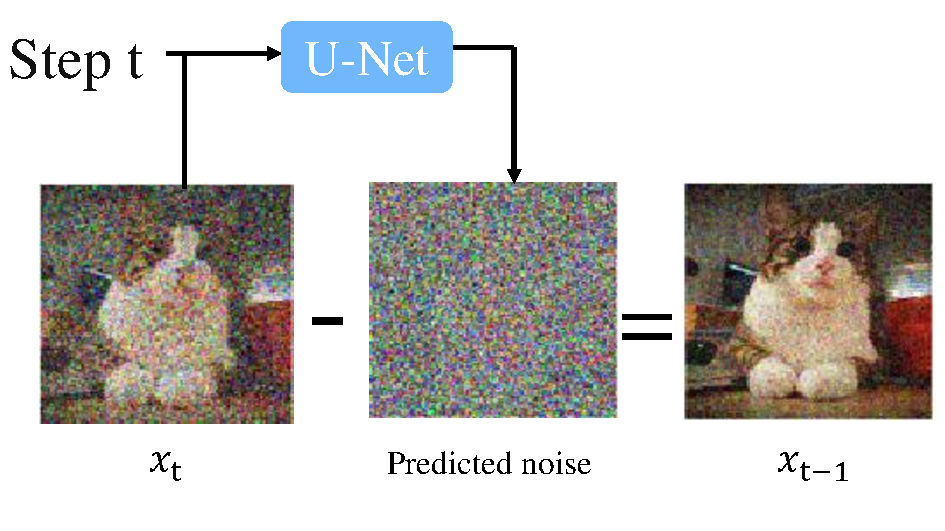
\includegraphics[width=12cm]{image/DDPM.pdf}
    \caption{DDPM single execution process}
    \label{fig:DDPM}
\end{figure}

As shown in Figure \ref{fig:DDPM}, at each step, by removing some of the noise, the current distribution evolves into the distribution for the next step. By performing multiple steps, the model learns how to generate samples (Generated image) that match the target data distribution from a simple distribution (Gaussian noise image), as shown in Figure \ref{fig:DDPM1}.
\begin{figure}[h]
    \centering
    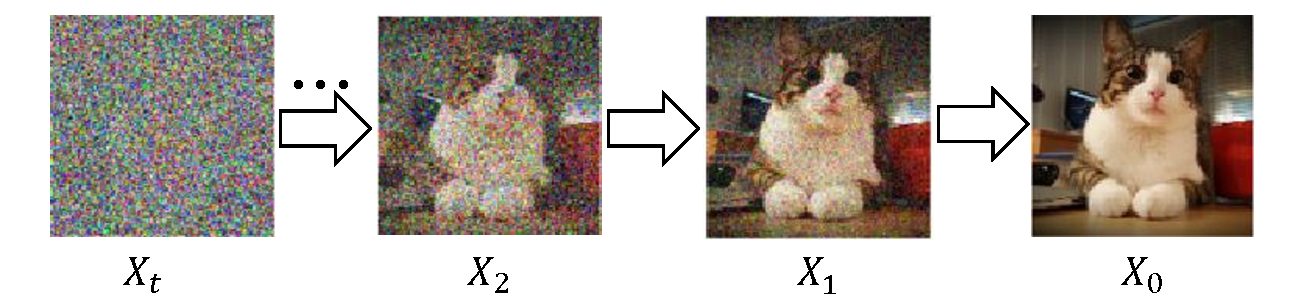
\includegraphics[width=14cm]{image/DDPM1.pdf}
    \caption{Image generation process for DDPM}
    \label{fig:DDPM1}
\end{figure}

Advantages of diffusion models is that they do not require adversarial training like Generative Adversarial Networks (GAN) \cite{goodfellow2020generative}, nor do they involve the complex inference processes of Variational Autoencoders (VAE) \cite{kingma2013auto}. This simplified training method makes diffusion probabilistic models easier to train in certain cases. GAN often face issues such as mode collapse and training instability, while VAE may involve high-dimensional integration calculations in their inference processes, adding to the complexity and difficulty of training the models. In contrast, diffusion models can be trained more smoothly and efficiently by gradually introducing noise and learning the denoising process.

U-Net is a convolutional neural network architecture for image segmentation tasks \cite{ronneberger2015u}. U-Net is inspired by the structure of the human eye and has two main parts, the encoder (down-sampling path) and the decoder (up-sampling path), and introduces jump connections. The encoder captures local features of the image by stacking convolutional and pooling layers to gradually reduce the spatial dimension of the input image. The decoder gradually recovers the spatial resolution of the image by upsampling and convolutional layers while incorporating feature information from the encoder. This allows the network to fuse different levels of feature information for better detail preservation and improved segmentation performance. Due to the excellent performance of U-Net, it is rapidly being used in various fields.

Since their initial proposal in 2015, diffusion probabilistic models have made significant advancements in backbone network structures. From the MLP used by Jascha in 2015 \cite{sohl2015deep}, to Song Yang's work in 2019 when he first constructed a diffusion model using the U-Net \cite{song2019generative}, and a series of improvements to the U-Net by subsequent works. Such as the DDPM \cite{ho2020denoising}, and the Imagen \cite{saharia2022photorealistic}. Imagen and many other works have made a series of improvements to U-Net. At present, most studies on diffusion probability modeling still use U-Net as the backbone network.

\section{Vision Transformer}
Vision Transformer model (ViT) \cite{dosovitskiy2020image} architecture typically consists of components such as a linear embedding layer, a self-attention layer, a fully-connected layer, a feed-forward layer, and residual connectivity with Layer Normalization.

Unlike traditional convolution-based approaches, Vision Transformer proposes a new paradigm for visual processing. The image is segmented into a series of fixed-size blocks, and the relationships between the blocks are established through a multi-head attention mechanism. The core of this idea is to view the image as a sequence rather than a grid, allowing the model to better capture global information while reducing the number of parameters and computational complexity.

The Multi-Head Attention mechanism allows the model to focus on information at different locations in parallel, effectively dealing with long-range dependencies. ViT performs well when dealing with large-scale image data, with a relatively small number of parameters compared to traditional convolutional networks, providing better scalability. Since it does not rely on a fixed local receptive field, ViT is more flexible in handling images of different sizes and application areas.

\section{AutoEncoderKL Model}
The Variational Autocoder (VAE) model with KL loss was developed by Diederik P. Kingma and Max Welling in Auto-Encoding Variational Bayes \cite{kingma2013auto}. This technique is used to generate continuous and smooth latent representations, often applied in fields like image generation, anomaly detection, and other generative tasks. As shown in Figure \ref{fig:AutoencoderKL}, The AutoencoderKL model typically consists of an encoder and a decoder. The encoder maps the data to a latent space representation, while the decoder reconstructs the data from the latent space representation, aiming to generate outputs that are similar to the original input.

\begin{figure}[h]
    \centering
    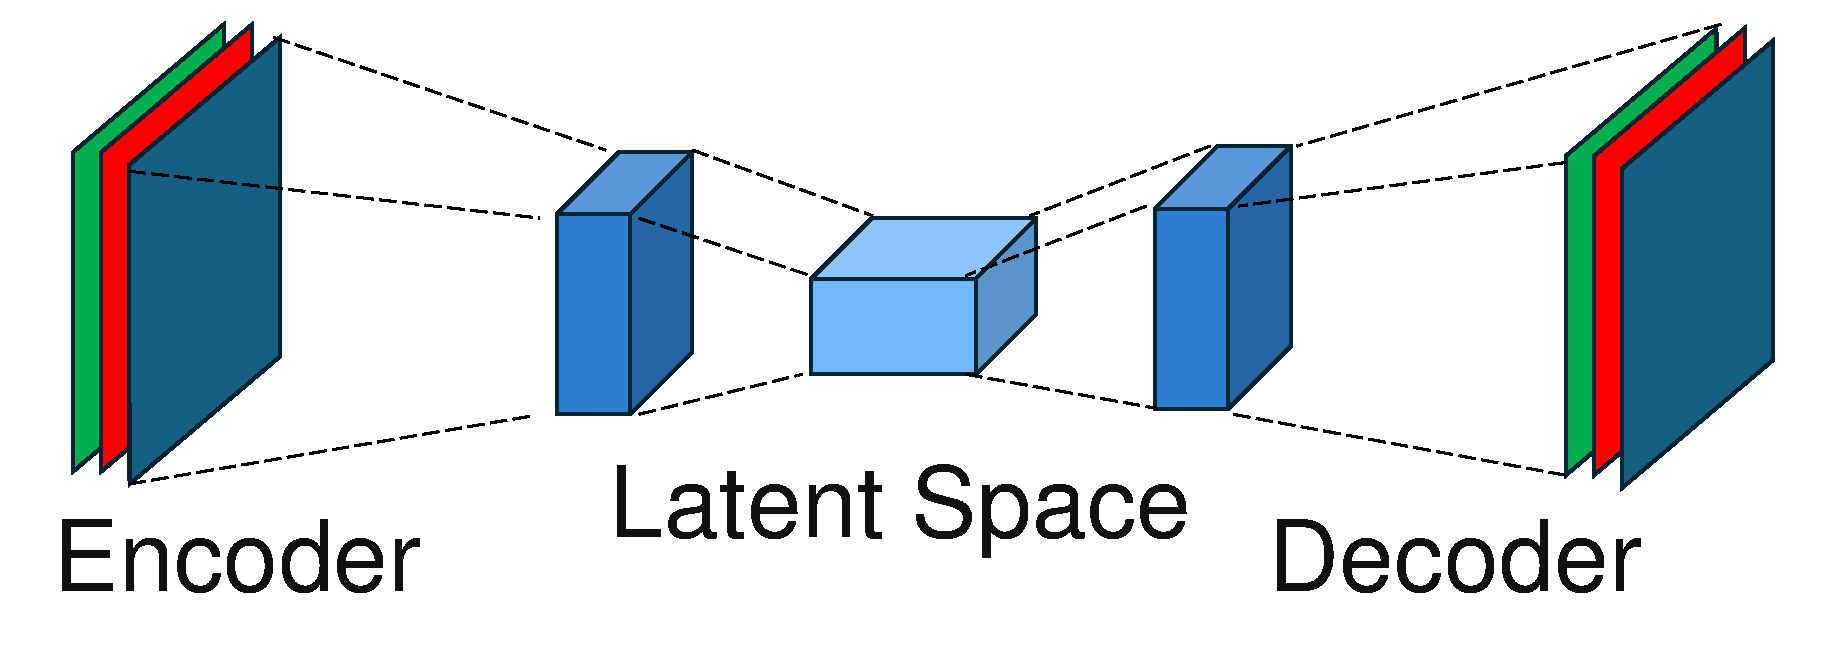
\includegraphics[width=12cm]{image/AutoencoderKL.pdf}
    \caption{AutoencoderKL model}
    \label{fig:AutoencoderKL}
\end{figure}

AutoencoderKL can be integrated into diffusion models to enhance their performance and capabilities. AutoencoderKL compresses data into a latent space representation, reducing dimensions while preserving essential features. This helps in effectively capturing the data distribution. By performing the diffusion process in the latent space instead of the high-dimensional data space, the model can operate more efficiently. The latent space typically has lower dimensions, making the diffusion process faster and computationally less expensive.
Since the AutoencoderKL model does not inherently participate in the generation of image semantics, it is typically not retrained repeatedly. The most commonly used AutoencoderKL pre-trained models are trained and released by Stability AI.
%同时KL散度项确保潜在空间分布保持平滑和连续,这对于生成高质量样本至关重要。它可以防止模型过度拟合并鼓励更好的泛化。
\section{Watercolor style image generation using GPU}
Before the widespread adoption of deep learning methods, a commonly used rendering algorithm in traditional computer graphics was dedicated to generating watercolor images. These early algorithms primarily created images by simulating the physical process of watercolor pigments flowing on study. The significant advantage of this approach is its ability to realistically reproduce the natural flow effects of watercolor pigments, resulting in highly realistic images.

However, this method also has some notable drawbacks, such as slow generation speed and the limitation to img2img tasks (i.e., converting an input image to an output image). To overcome the slow generation speed, researchers attempted to accelerate the algorithm using parallel computing tools like CUDA. Despite improvements in speed, this method still relied on input images to generate watercolor images, greatly limiting the model's expressive capabilities and flexibility. This limitation not only constrained the algorithm in generating diverse watercolor styles but also rendered it inadequate for meeting the increasingly diverse demands of artistic creation in practical applications.
%同时,深度学习模型训练需要大量的训练用图像。可以利用该方法生成大量训练用图像。
%\section{local Feed Forward}
\chapter{Dataset}
\section{Watercolor Dataset}
The watercolor dataset used in this study was personally collected based on the ImageNet dataset. ImageNet is a large scale image dataset initially created by Fei-Fei Li and others at Stanford University. It contains over a million high-resolution images spanning a thousand different categories, with each category typically including hundreds to thousands of images \cite{deng2009imagenet}. 

In this study, images from selected categories of the ImageNet dataset were converted to watercolor images using GPU methods. Ultimately, the resulting dataset comprised 35 categories (as shown in Table \ref{tab:35categories} for specific categories), each with approximately 2,000 images. Each image had a resolution of 512$\times$512, and the total dataset included 68,550 images.
\begin{table}[htbp]
  \centering
  \caption{The 35 categories extracted from the ImageNet dataset.}
  \label{tab:35categories}
  \begin{tabular}{c c|c c}
    No&Name&No&Name  \\
    \hline
    n02085620 & Chihuahua             & n02127052 & Rule          \\
    n02085782 & Japanese Spaniel      & n04118776 & Schooner      \\
    n02085936 & Maltese Dog           & n04147183 & Trimaran      \\
    n02086079 & Pekingese             & n04483307 & Trimaran      \\
    n02086240 & Shih Tzu              & n04612504 & Yawl          \\
    n02086646 & King Charles Spaniel  & n04613696 & Yurt          \\
    n02123045 & Tabby                 & n09193705 & Snow Mountain \\
    n02123159 & Tiger                 & n09229709 & Bubble        \\
    n02123394 & Persian Cat           & n09246464 & Cliff         \\
    n02123597 & Siamese Cat           & n09256479 & Coral Reef    \\
    n02124075 & Egyptian Cat          & n09288635 & Geyser        \\
    n02125311 & Cougar                & n09332890 & Lakeside      \\
    n09399592 & Promontory            & n09421951 & Promontory    \\
    n09428293 & Beach                 & n09468604 & Valley        \\
    n09472597 & Volcano               & n12985857 & Coral Fungus  \\
    n12998815 & Agaric                & n13037406 & Gyromitra     \\
    n13040303 & Stinkhorns            & n13044778 & Earth Stars   \\
    n13052670 & Grifola Frondosa      &           &               \\
  \end{tabular}
\end{table}




%\begin{table}[htbp]
%  \centering
%  \caption{The 35 categories extracted from the ImageNet dataset.}
%  \label{tab:35categories}
%  \begin{tabular}{c c|c c|c c}
%    No&Name&No&Name&No&Name  \\
%    \hline
%    n02085620 & Chihuahua             & n02127052& Rule          &n09399592&Promontory  \\
%    n02085782 & Japanese Spaniel      & n04118776& Schooner      &n09421951&Promontory \\
%    n02085936 & Maltese Dog           & n04147183& Trimaran      &n09428293&Beach \\
%    n02086079 & Pekingese             & n04483307& Trimaran      &n09468604&Valley \\
%    n02086240 & Shih Tzu              & n04612504& Yawl          &n09472597&Volcano \\
%    n02086646 & King Charles Spaniel  & n04613696& Yurt          &n12985857&Coral Fungus \\
%    n02123045 & Tabby                 & n09193705& Snow Mountain &n12998815&Agaric \\
%    n02123159 & Tiger                 & n09229709& Bubble        &n13037406&Gyromitra \\
%    n02123394 & Persian Cat           & n09246464& Cliff         &n13040303&stinkhorns \\
%    n02123597 & Siamese Cat           & n09256479& Coral Reef    &n13044778&Earth stars \\
%    n02124075 & Egyptian Cat          & n09288635& Geyser        &n13052670&Grifola Frondosa \\
%    n02125311 & Cougar                & n09332890& Lakeside      \\
%  \end{tabular}
%\end{table}

\section{Methods of Dataset Collection }
Due to the current lack of open-source watercolor datasets, this study used GPU methods to collect watercolor images as the dataset. The GPU method itself does not depend on a specific dataset, meaning it can convert input images into watercolor images. This method can simulate relatively realistic watercolor effects but still requires input images.

In this study, the dataset images were collected using this method, and the specific process is Figure \ref{fig:gpu}. First, the resolution of images from the ImageNet dataset was increased from 256$\times$256 to 512$\times$512. This is because the performance of the aforementioned GPU method deteriorates significantly at lower resolutions. Then, the images with the increased resolution were converted into watercolor images using the GPU method. This resulted in watercolor images along with their corresponding original ImageNet images.

\begin{figure}[h]
    \centering
    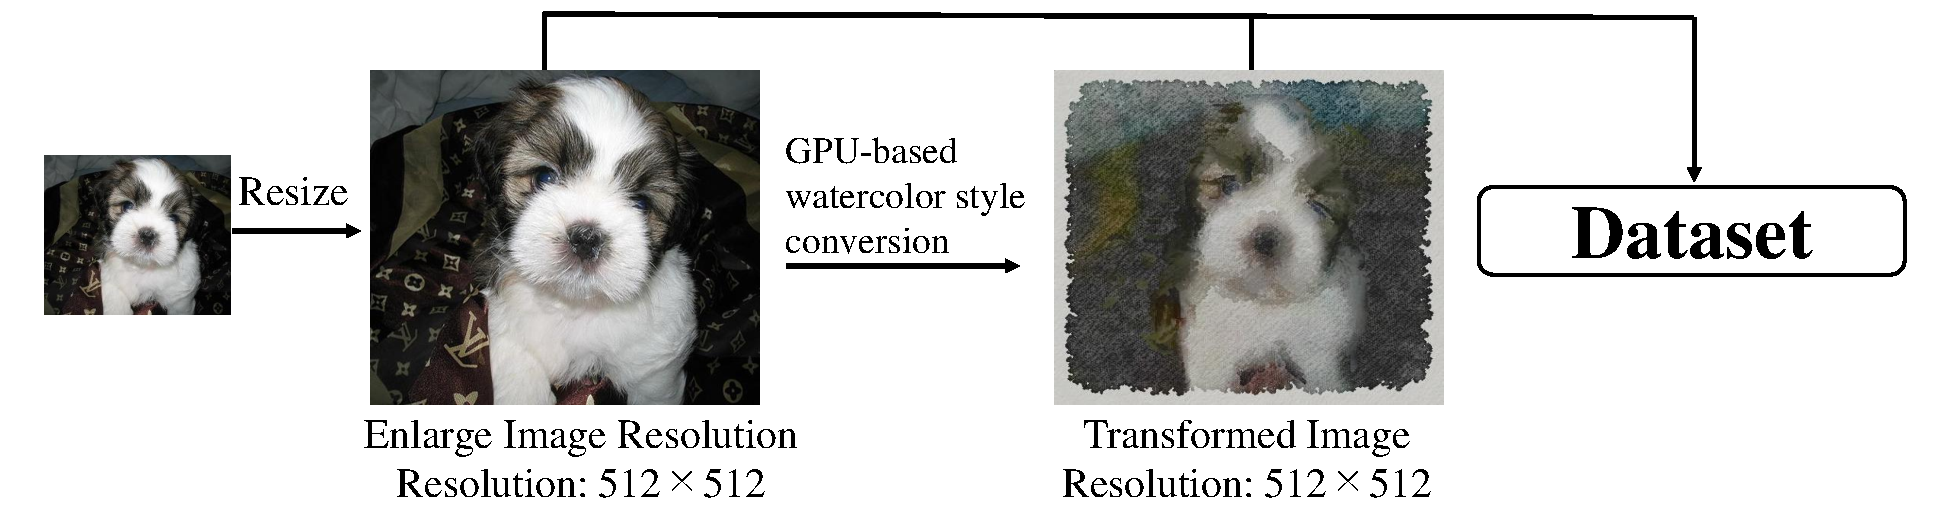
\includegraphics[width=16cm]{image/gpu.pdf}
    \caption{The process of watercoloring ImageNet image}
    \label{fig:gpu}
\end{figure}

\section{Modification of Datasets}
To ensure the model retains more semantic information during the generation process, we adopted a unique approach when constructing the dataset. This approach involves using both watercolor styled images and the original ImageNet images. Specifically, this means that for each category, the dataset includes not only the original images but also their corresponding watercolor styled images. These images appear in pairs, as shown in Figure \ref{fig:pairs}. This dual image processing method helps the model better understand and retain key semantic features during training, thereby improving the quality and accuracy of the generated results.
%通过混合两种类型的图像,希望模型在数据集内学习到水彩风格的同时,提升图像语义的

\begin{figure}[h]
    \centering
    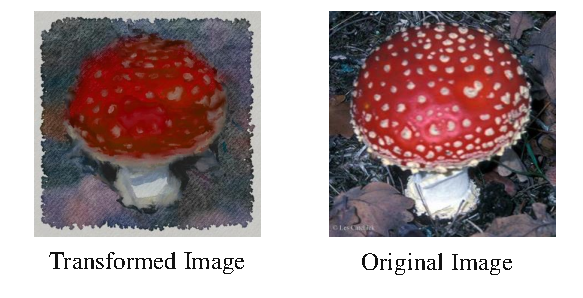
\includegraphics[width=14cm]{image/pairs.pdf}
    \caption{The image pair in the dataset (Agaric)}
    \label{fig:pairs}
\end{figure}


\chapter{Proposed Method}
\section{Overall Structure}
To achieve the goal of generating high-quality images and reducing the computational load of the model, this study's model comprises two networks. As shown in Figure \ref{fig:overall}, the Transformer model and the AutoencoderKL model. During the image generation process, the Transformer model first generates specific feature maps from random noise, guided by labels. Then, the AutoencoderKL model decodes these feature maps generated by the Transformer model into images.

\begin{figure}[h]
    \centering
    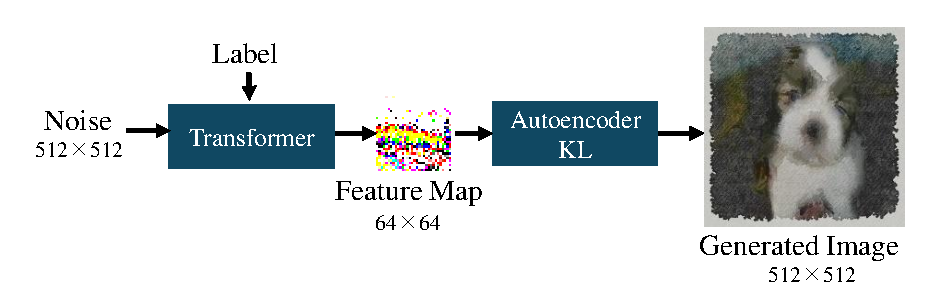
\includegraphics[width=16cm]{image/overall.pdf}
    \caption{Overall structure}
    \label{fig:overall}
\end{figure}

The introduction of the AutoencoderKL model transforms the diffusion model from pixel-level generation (directly generating images) to latent space generation (generating feature maps). Therefore, the training or inference of the diffusion model with the AutoencoderKL model essentially takes place on feature maps. This significantly reduces the computational load required for training the diffusion model. Additionally, the AutoencoderKL model helps prevent overfitting to some extent and provides smoother outputs.

It is worth mentioning that during the model inference process, only the encoder part of the AutoencoderKL model is involved, i.e., it is used to restore the feature maps. The decoder module of the AutoencoderKL model plays a more significant role during model training.

\section{Transformer Model}
To generate high-quality watercolor images, this study abandoned the commonly used U-Net network in traditional diffusion models and instead reconstructed a network based on the Vision Transformer model as the backbone of the diffusion model, as shown in Figure \ref{fig:traM}. The Attention structure of the Transformer model possesses stronger global perception capabilities, a feature particularly important in the process of generating watercolor images. By leveraging this structure, the watercolor image generation process can more effectively simulate the diffusion and blending effects of watercolor pigments, thereby enhancing the overall texture and detail expressiveness of the images. Compared to traditional methods, the Vision Transformer-based network not only excels in simulating watercolor effects but also significantly improves the quality and realism of the generated images.

\begin{figure}[htbp]
    \centering
    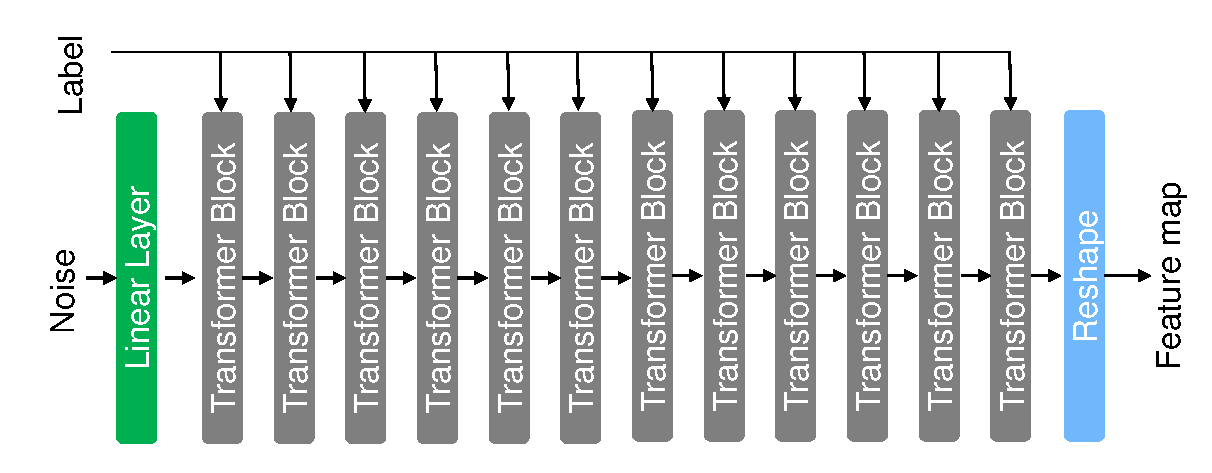
\includegraphics[width=16cm]{image/traM.pdf}
    \caption{Transformer model structure}
    \label{fig:traM}
\end{figure}

The design of the Transformer model generally adopts a relatively simple linear structure. This design, with similar structures at each layer, facilitates the model's expansion and improvement and offers higher efficiency in parallel computation.

Since data in the Transformer structure is computed in vector form, Linear Layers and Reshape operations are added to the input and output sections to convert the original matrices into vectors. In the main body of the model, 12 Transformer Blocks are stacked and reused. To enhance the model's control over different types of images and generate images with higher recognizability, label information is input into each Transformer Block.

\section{Transformer Block}
The design of the Transformer Block generally follows the linear structure of the traditional Vision Transformer, as shown in Figure \ref{fig:Transformer_Block}. The difference in this study's Transformer Block design is the replacement of the original MLP layer with a Feed-Forward layer, using the MLP to input label information. To improve the model's performance, the number of Multi-Head Attention layers (MH-Attention) was increased, and the Multi-Head Attention layers and Feed-Forward layers were used in pairs. This is because the Multi-Head Attention layer has relatively weak local perception and non-linear capabilities, which are compensated for by the Feed-Forward layer. The Multi-Head Attention layer, through the parallel processing of multiple attention heads, can better capture the global information of the input data. Meanwhile, the Feed-Forward layer, through non-linear transformations, enhances the model's ability to handle complex patterns and features.

\begin{figure}[thbp]
    \centering
    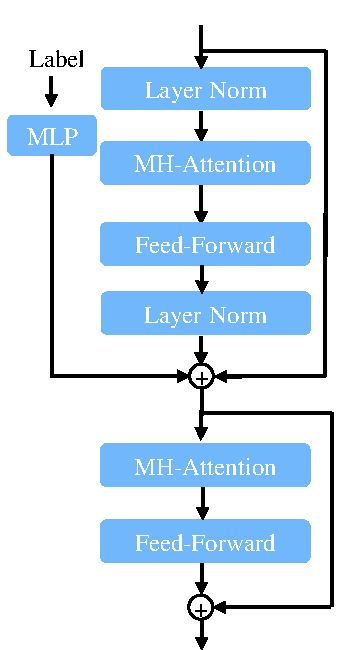
\includegraphics[width=7cm]{image/Transformer_Block.pdf}
    \caption{Transformer block structure}
    \label{fig:Transformer_Block}
\end{figure}

This design approach is based on the optimization of combining the respective strengths and weaknesses of the Multi-Head Attention layer and the Feed-Forward layer. The Multi-Head Attention layer excels at capturing global dependencies in the input data but is somewhat deficient in handling local information and non-linear transformations. Conversely, the Feed-Forward layer is adept at local perception and non-linear transformations. By supplementing each other, the entire Transformer Block becomes more balanced and comprehensive in information processing and feature extraction. A detailed introduction to the Feed-Forward layer will be provided in the next section.
\section{Feed Forward Layer Module }
The structure of the Feed Forward Layer designed in this study is shown in Figure \ref{fig:FFL}. The main function of the Feed Forward Layer is to compensate for the shortcomings of the Attention layer in terms of non-linear capability and local perception.

\begin{figure}[thbp]
    \centering
    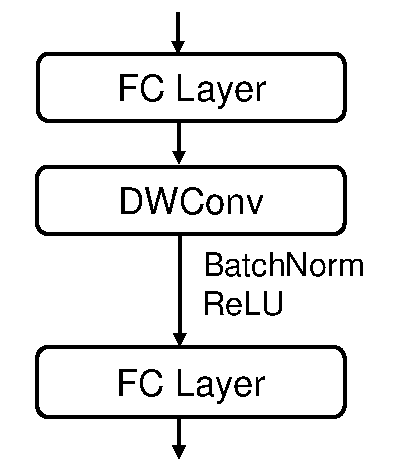
\includegraphics[width=8cm]{image/FFL.pdf}
    \caption{Feed Forward Layer structure}
    \label{fig:FFL}
\end{figure}

%总的来说,Feed Forward Layer 的设计通过 ReLU 激活函数和卷积操作的引入,增强了模型的非线性表征能力和局部感知能力。而在正规化方法上选择 Batch Norm + ReLU 组合,则进一步提升了模型在卷积计算中的表现和训练效率。使用 DWConv 代替标准卷积,则有效地控制了计算成本,使得模型在实际应用中更加高效。通过这种综合优化的设计,Feed Forward Layer 能够更好地适应不同任务需求,提升 Transformer 模型的整体性能。
Specifically, the introduction of the ReLU activation function allows the model to better handle complex non-linear relationships, while convolution operations enhance the model's ability to capture local features.

Due to the introduction of convolution computations, We chose a different Normalization method compared to the commonly used Layer Normalization + SiLU combination in Transformer models. Instead, opted for the Batch Normalization + ReLU combination, which is more commonly used in convolutional neural networks. Batch Normalization can more effectively handle the changes in data distribution brought about by convolution operations, thereby improving the model's training stability and convergence speed. To address the increased computational load brought by convolution operations, Depthwise Convolution (DW Conv) was used in the Feed Forward Layer instead of standard convolution. Depthwise Convolution performs convolution operations independently on each channel, significantly reducing the number of parameters and computational load, thereby improving computational efficiency while maintaining model performance.

\begin{figure}[thbp]
    \centering
    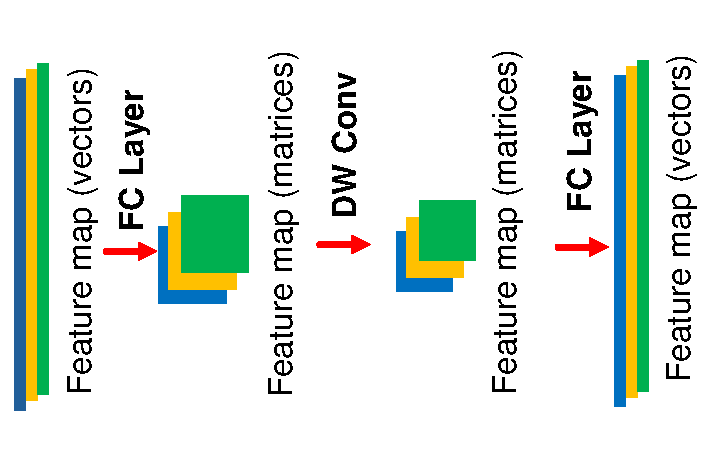
\includegraphics[width=14cm]{image/FFL1.pdf}
    \caption{Feature map transformation process (Example with 3 channels)}
    \label{fig:FFL1}
\end{figure}

It's worth mentioning that since data in the Transformer is in vector form, direct convolution operations are not feasible. Therefore, some preprocessing steps are required in the Feed Forward Layer to facilitate convolution calculations. First, a Fully Connected Layer (FC Layer) is used to convert the input vector into a matrix form. This step aims to expand the originally one-dimensional vector data into two-dimensional matrix data, giving it the structure needed for convolution operations. After performing the convolution calculations, It's important to note that because Depthwise Convolution does not change the number of data channels, no additional operations are needed to modify the channel count. Finally, another Fully Connected Layer converts the matrix back into vector form. Through this process, the data is transformed from matrix form back to vector form, allowing it to seamlessly connect with the rest of the Transformer. As shown in Figure \ref{fig:FFL1}.

In summary, the Feed Forward Layer handles convolution computations by first converting vectors into matrix form, then extracting features through convolution operations, and finally converting the matrix back into vector form. This series of steps not only enables the implementation of convolution calculations within the Transformer but also ensures an enhancement in model performance.

\section{MLP Module }
MLP (Multilayer Perceptron) is a simple neural network structure, usually consisting of several fully connected layers and activation functions. In the original Vision Transformer, an MLP was often connected after the Attention layer to introduce nonlinear capabilities to the model.

\begin{figure}[thbp]
    \centering
    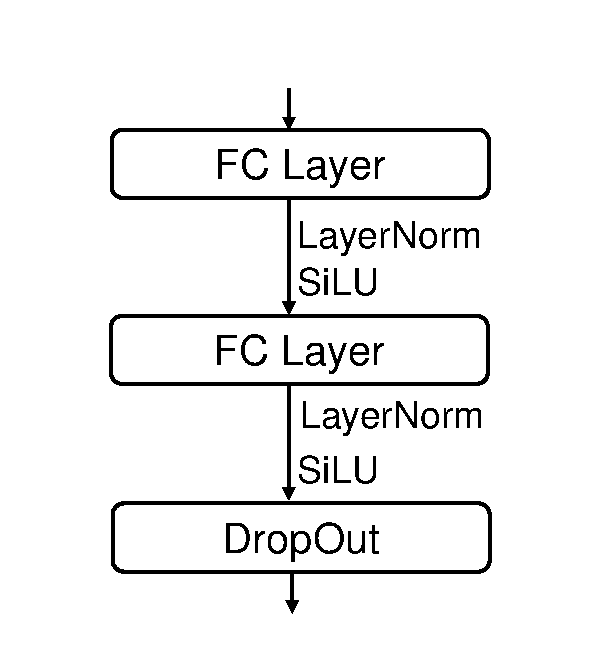
\includegraphics[width=9cm]{image/MLP.pdf}
    \caption{MLP structure}
    \label{fig:MLP}
\end{figure}

In this study, an MLP is used to input label data into the model. The structure of the MLP is shown in Figure \ref{fig:MLP}. This MLP structure adopts a combination of fully connected layers and Layer Normalization + SiLU. The reason for choosing this structure is that, in Transformer models, theLayer Normalization + SiLU combination performs better in processing vector data.

Layer Normalization (Layer Norm) is used to standardize the input data, making the mean zero and variance one for each training batch. It also stabilizes the model's training performance and reduces the adverse effects caused by changes in data distribution. The SiLU (Sigmoid Linear Unit) activation function combines the advantages of ReLU and Sigmoid, providing good non-linear transformation capabilities. Unlike ReLU, which clips negative inputs to zero, SiLU allows negative information to pass through, preserving the integrity of these values and thereby improving the model's expressive power.

In summary, the fully connected layers are responsible for linear transformations, mapping the input label data to a higher-dimensional feature space for subsequent processing. The data after the fully connected layers is standardized by Layer Normalization and then undergoes non-linear transformation through the SiLU activation function, thereby enhancing the model's expressive power.


\chapter{Experiments}
\section{Train Details }
To train this model, NVIDIA RTX A6000$\times$2 was used. and the batch size was set to 16, the learning rate was 1e-4, and the optimizer was selected as AdamW. A total of 1500 epochs were trained, and checkpoints were saved at every 300 epochs. The AutoencoderKL version used in this study is vae-ft-mse-840000-ema-pruned.safetensors.
\section{Valuation Metric}\label{chap:ValuationMetric}
Regarding evaluation metrics, this study uses FID (Fréchet Inception Distance) \cite{FID} as an objective evaluation metric. Additionally, questionnaire are used as a subjective evaluation metric. In comparison with other diffusion models, the above metrics will be used.

FID was initially used as a metric to evaluate the quality of images generated by Generative Adversarial Networks. It measures the quality of generated images by comparing the distribution differences between generated images and real images in feature space. First, a pre-trained Inception V3 model is used to extract features from both real and generated images. The extracted features are then represented as distributions in a high-dimensional space. Finally, the FID quantifies the difference between real and generated images by calculating the Fréchet distance between the distributions of the real and generated image features. The calculation formula is shown in Equation \ref{eq:fid}.

\begin{equation} \label{eq:fid}
\text{FID} = \left\| \mu_r - \mu_g \right\|^2 + \text{Tr}\left( \Sigma_r + \Sigma_g - 2(\Sigma_r\Sigma_g)^{1/2} \right)
\end{equation}

where:
\begin{itemize}
  \item \(\mu_r\) and \(\Sigma_r\) are the mean and covariance matrix of the real images' features.
  \item \(\mu_g\) and \(\Sigma_g\) are the mean and covariance matrix of the generated images' features.
  \item \(\text{Tr}\) denotes the trace of a matrix.
\end{itemize}

FID provides a numerical metric to quantify the similarity between generated images and real images, and it is widely used in evaluating the quality of generated images.

Regarding the questionnaire, the proposed model, Denoising Diffusion Probabilistic Models(DDPM), and Latent Diffusion Model (LDM) models are first trained and used to generate images under the same conditions.As shown in Figure\ref{fig:questionnaire}, This questionnaire contains a total of ten questions, each corresponding to a category of watercolor images generated by the models. Each question presents 9 images (three generated by each model), and respondents are asked to choose the top three images that best represent the watercolor style. The first choice receives 3 points, the second choice receives 2 points, and the third choice receives 1 point. The final survey score for each model is then calculated based on these points.
\begin{figure}[thbp]
    \centering
    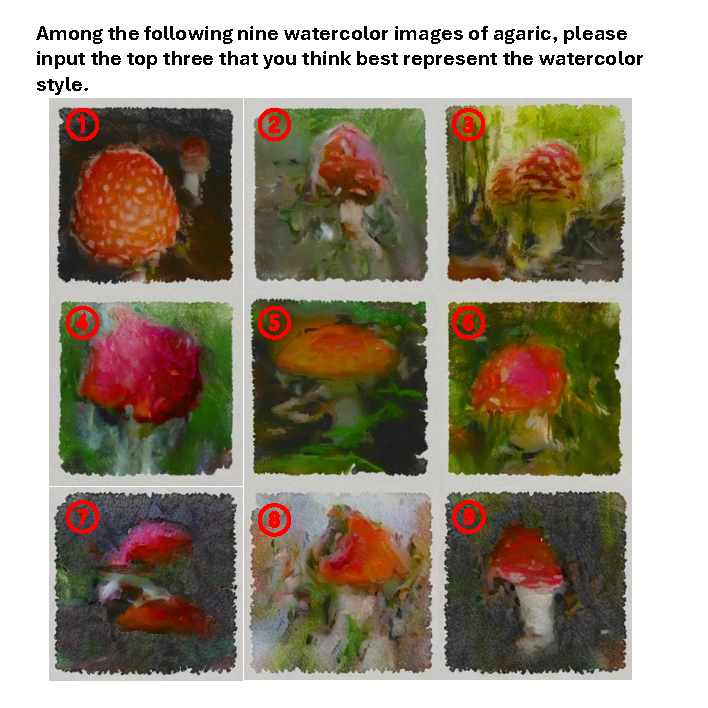
\includegraphics[width=13cm]{image/questionnaire.pdf}
    \caption{Questionnaire example}
    \label{fig:questionnaire}
\end{figure}
\section{Result Analysis}
The features of watercolor images include special effects such as color blending and blooming,as shown in Figure \ref{fig:tureImage}. Color blending refers to the natural mixing of colors on the study in watercolor painting, forming new colors. This blending is usually incomplete, allowing both the original and mixed colors to coexist. The blooming effect is characterized by the high water content of watercolor pigments, causing them to seep into the study fibers and produce a distinctive blooming effect. This effect is often used to depict skies, oceans, and other natural landscapes.

\begin{figure}[htbp]
    \centering
    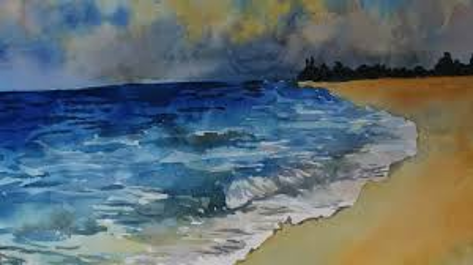
\includegraphics[width=14cm]{image/tureImage.png}
    \caption{Real watercolor results (Beach)}
    \label{fig:tureImage}
\end{figure}

Using the model in this study, images were generated under the aforementioned training conditions (e.g., a beach image), as shown in Figure \ref{fig:ResultAnalysis}. By comparing these with real watercolor images in Figure \ref{fig:tureImage}, it can be seen that the model's generated results successfully mimic the characteristics of watercolor images. 

In the red-circled areas, there is a noticeable color blending effect where the ochre and light blue colors merge to form a shade similar to light gray, closely resembling the effect of real watercolor pigment blending. In the yellow-circled areas, a clear blooming effect can be observed, where the edges of the clouds and sky show a smooth transition. This simulates the flow of pigments in watercolor painting.
\newpage
\begin{figure}[htbp]
    \centering
    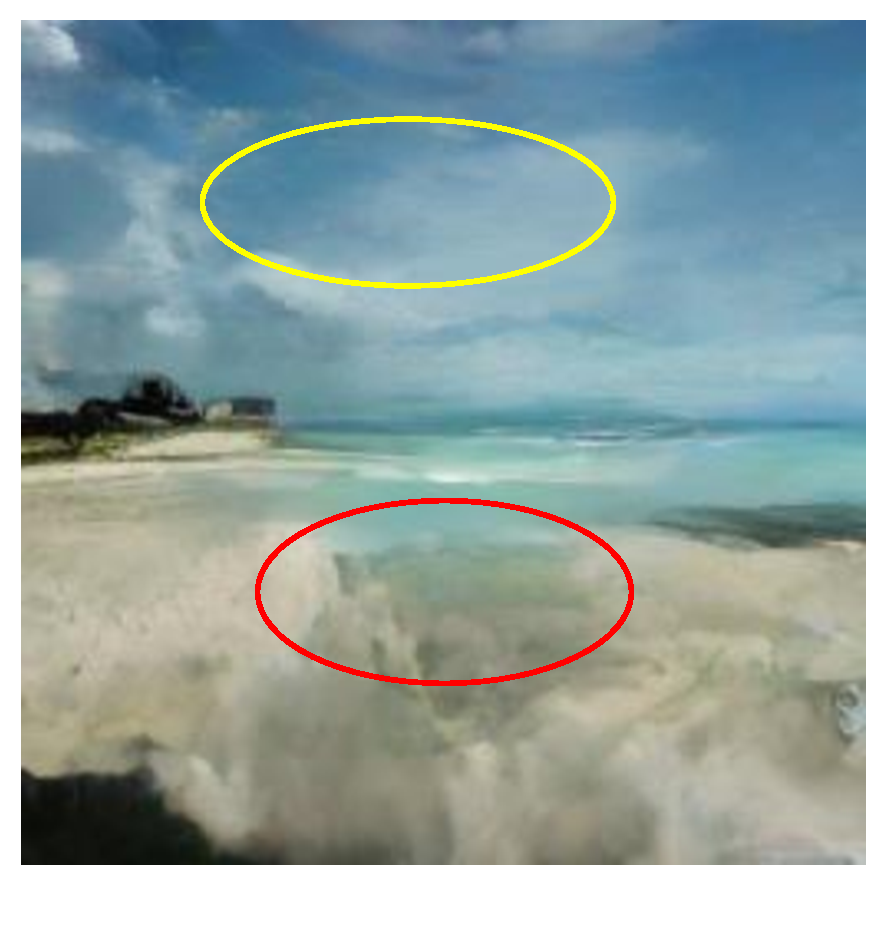
\includegraphics[width=15cm]{image/ResultAnalysis.pdf}
    \caption{Generated results (Beach)}
    \label{fig:ResultAnalysis}
\end{figure}

\section{Comparison with GPU method}
%这里对比GPU方法
%文字说明可以再改一下
In the previous section, a GPU method was used to generate the dataset \cite{huang2021gpu},
comparison of the generated images was carried out. The image style conversion by GPU method (green box is original image). and generated images with using the model in this paper. Approximate images were generated for ease of comparison (beach image). As shown in Figure \ref{fig:wGPU}.

\begin{figure}[htbp]
    \centering
    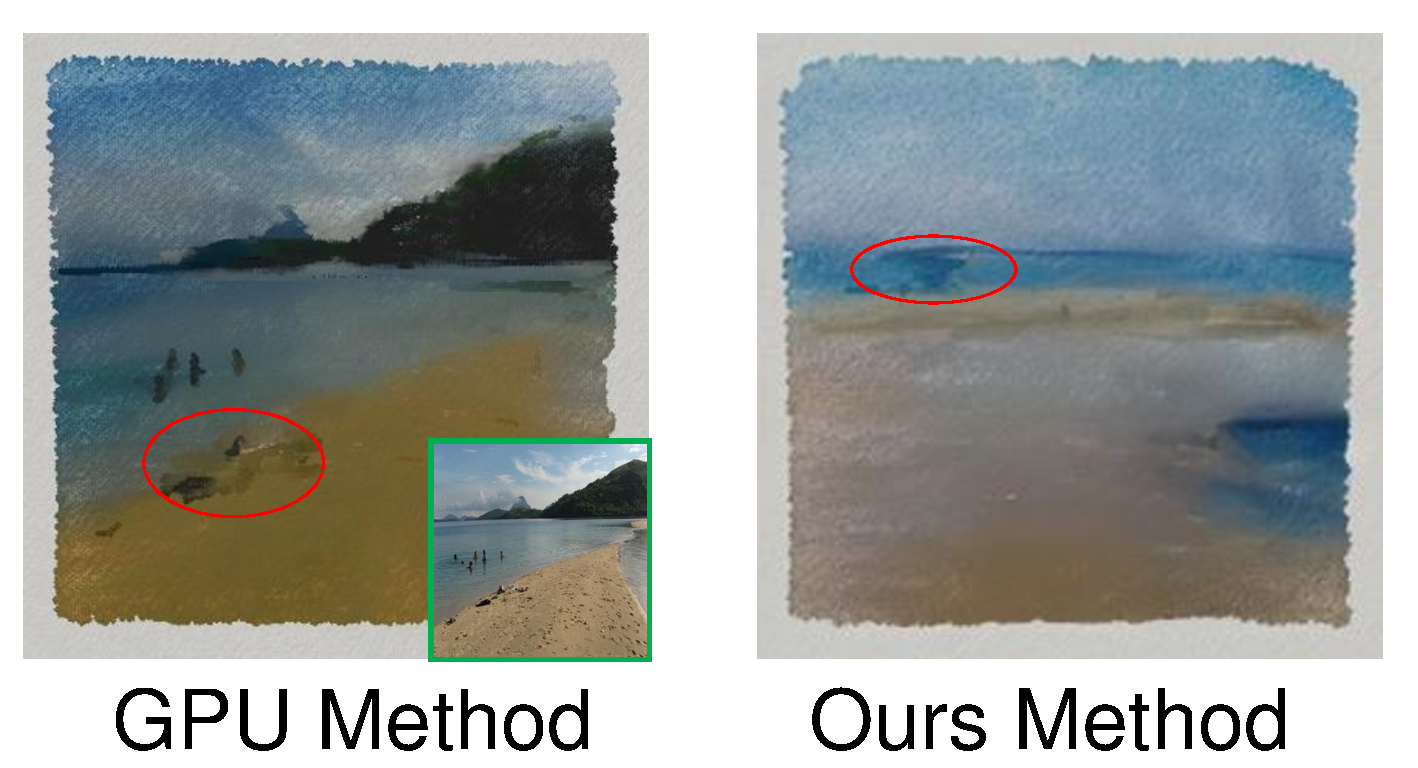
\includegraphics[width=13cm]{image/wGPU.pdf}
    \caption{Comparison of the generated image with GPU generation method (Beach)}
    \label{fig:wGPU}
\end{figure}

Compared to the GPU method-generated images, the model excels particularly in color blending, especially in the red-circled areas, showcasing the natural merging effect characteristic of watercolor paintings. Additionally, the blurred edges in the image make the overall picture softer and more realistic. The model also successfully replicates the texture effects of watercolor paintings present in the dataset, making the generated images more artistic and visually appealing. Overall, the model demonstrates excellent reconstruction capability of the dataset, accurately capturing the artistic features of watercolor images.
\section{Comparison with DDPM and LDM}
%这里对比其他模型,并分析评价指标。

To compare with existing research, the Frechet Inception Distance (FID) \cite{FID} was used to objectively evaluate the results generated by the model. As shown in Table \ref{tab:fid}, our model achieved the lowest FID score compared to the original Denoising Diffusion Probabilistic Model (DDPM) \cite{ho2020denoising} and the Latent Diffusion Model (LDM) \cite{rombach2022high}. This indicates that our model's generated images are the closest to real images in terms of quality and diversity, outperforming the existing DDPM and LDM models.

\begin{table}[htbp]
  \centering
  \caption{Objective evaluation}
  \label{tab:fid}
  \begin{tabular}{c c}
    \hline
    Model & FID  \\
    \hline
    Denoising Diffusion Probabilistic Models & 73.933  \\
    Latent Diffusion Models & 67.261\\
    Ours & 64.332  \\
    \hline
  \end{tabular}
\end{table}

In terms of subjective evaluation, this study collected a total of 11 valid questionnaires, and the results were compiled according to the method described in Section \ref{chap:ValuationMetric}. Respondents rated the images generated by different models based on their watercolor style (Total score 660), as shown in Table \ref{tab:point}. The results in Table \ref{tab:point} indicate that the DDPM model's score is significantly lower compared to the other models, with a score of 143. In contrast, the LDM model received a score of 220, while our model slightly outperformed the LDM model in user ratings, achieving a score of 297. These results are consistent with the objective FID evaluation and further validate the superiority of our model in generating high-quality watercolor images from the users' perspective. These subjective evaluation results further demonstrate the advantages of our model in generating watercolor images.
%分数
\begin{table}[htbp]
  \centering
  \caption{Subjective evaluation}
  \label{tab:point}
  \begin{tabular}{c c}
    \hline
    Model & Sum Points  \\
    \hline
    Denoising Diffusion Probabilistic Models & 143  \\
    Latent Diffusion Models & 220  \\
    Ours & 297  \\
    \hline
  \end{tabular}
\end{table}

% \begin{table}[htbp]
%   \centering
%   \caption{Objective evaluation}
%   \label{tab:fid1}
%   \begin{tabular}{c c c c }
%     \hline
%     Label & Ours & DDPM & LDMs \\
%     \hline
%     Agaric & 5 & 0 & 2 \\
%     coast & 55.632 & DDPM & LDMs \\
%     beach & 55.632 & DDPM & LDMs \\
%     Siamese_cat & 55.632 & DDPM & LDMs \\
%     geyser   & 55.632 & DDPM & LDMs \\
%     Snow mountain & 55.632 & DDPM & LDMs \\
%     Valley & 55.632 & DDPM & LDMs \\
%     volcano & 55.632 & DDPM & LDMs \\
%     lakeside     & 55.632 & DDPM & LDMs \\
%     yawl & 55.632 & DDPM & LDMs \\
%     \hline
%   \end{tabular}
% \end{table}


Comparing the above three models generates images (Agaric) as shown in Figure \ref{fig:eva}. The model in this study achieved the best watercolor simulation subjectively. Looking closely at the generation results, this study's model has a better reconstruction of the target within the image, and the unique features of watercolor images such as color diffusion and color fusion appear at the line edges of the image. Moreover, the generated image has fewer meaningless lines and color blocks and shows light and shadow effects to some extent. To further test the effectiveness of the model in this study, more categories of images were generated, as shown in Figure \ref{fig:more}.
\begin{figure}[h]
    \centering
    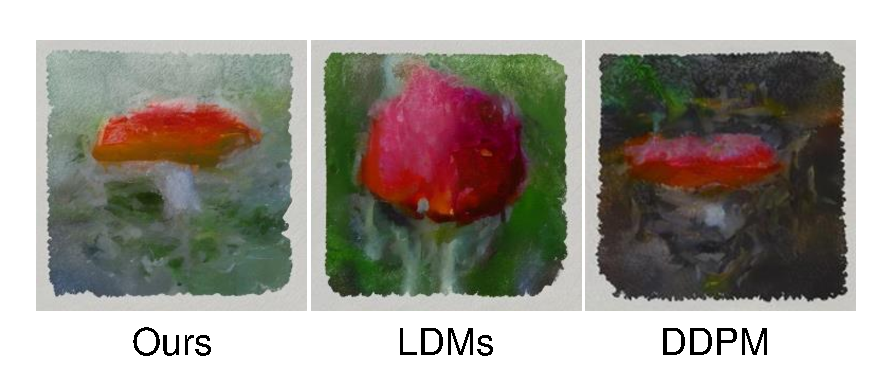
\includegraphics[width=16cm]{image/eva.pdf}
    \caption{Comparison of the generated image (Agaric)}
    \label{fig:eva}
\end{figure}

\newpage
\begin{figure}[thbp]
    \centering
    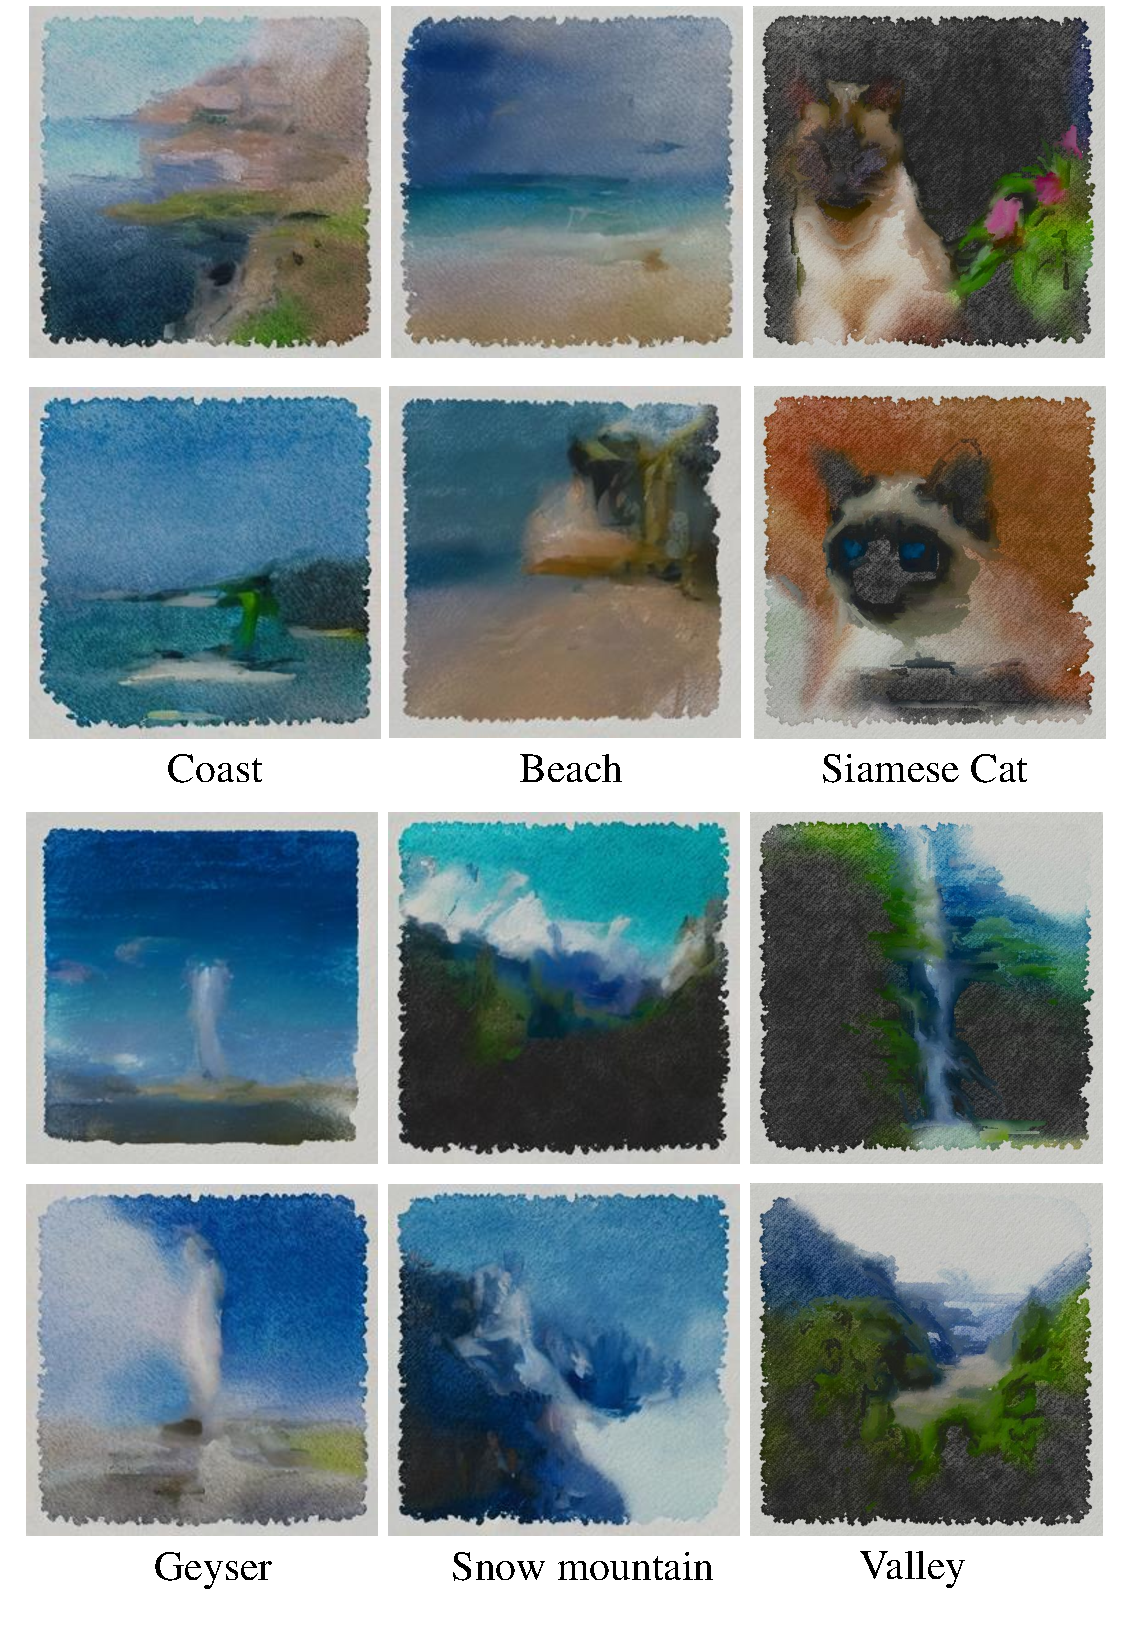
\includegraphics[width=15cm]{image/more.pdf}
    \caption{More categories of generated results}
    \label{fig:more}
\end{figure}

\chapter{Conclusion}
In this study, we created a high-quality watercolor dataset and designed a neural network based on the Transformer architecture specifically for watercolor image generation. The detailed design of the model's framework allows for the generation of images according to labels. The generated images retain the characteristics of watercolor paintings, such as color blending and diffusion effects. Both objective metrics and subjective evaluations indicate that the performance of our model in generating watercolor images slightly surpasses that of popular diffusion models based on the U-Net structure.

%%%%%%%%%%%%%%%%%%%%%%%%%%%%
%%%%    謝辞    %%%%
%%%%%%%%%%%%%%%%%%%%%%%%%%%%
\chapter*{Acknowledgement}
I would like to express my sincere thanks to Prof. Koji Nakano, Prof. Yasuaki Ito, and Assistant Prof. Satoki Tsuji for their enthusiastic guidance and valuable comments and suggestions during their busy schedules. I also express our sincere gratitude to all the members of the laboratory.



%%%%%%%%%%%%%%%%%%%%%%%%%%%%
%%%%   参考文献   %%%%
%%%%%%%%%%%%%%%%%%%%%%%%%%%%
\bibliographystyle{IEEEtran}
\bibliography{sample}

\end{document}
